\documentclass[../../main.tex]{subfiles}
\graphicspath{{\subfix{../../diagrams/}}}
\usepackage{lipsum}  
\usepackage{float}

\begin{document}
\begin{figure}[h!]
\caption{Delivery module class diagram.}
\vspace{10mm}
\centering
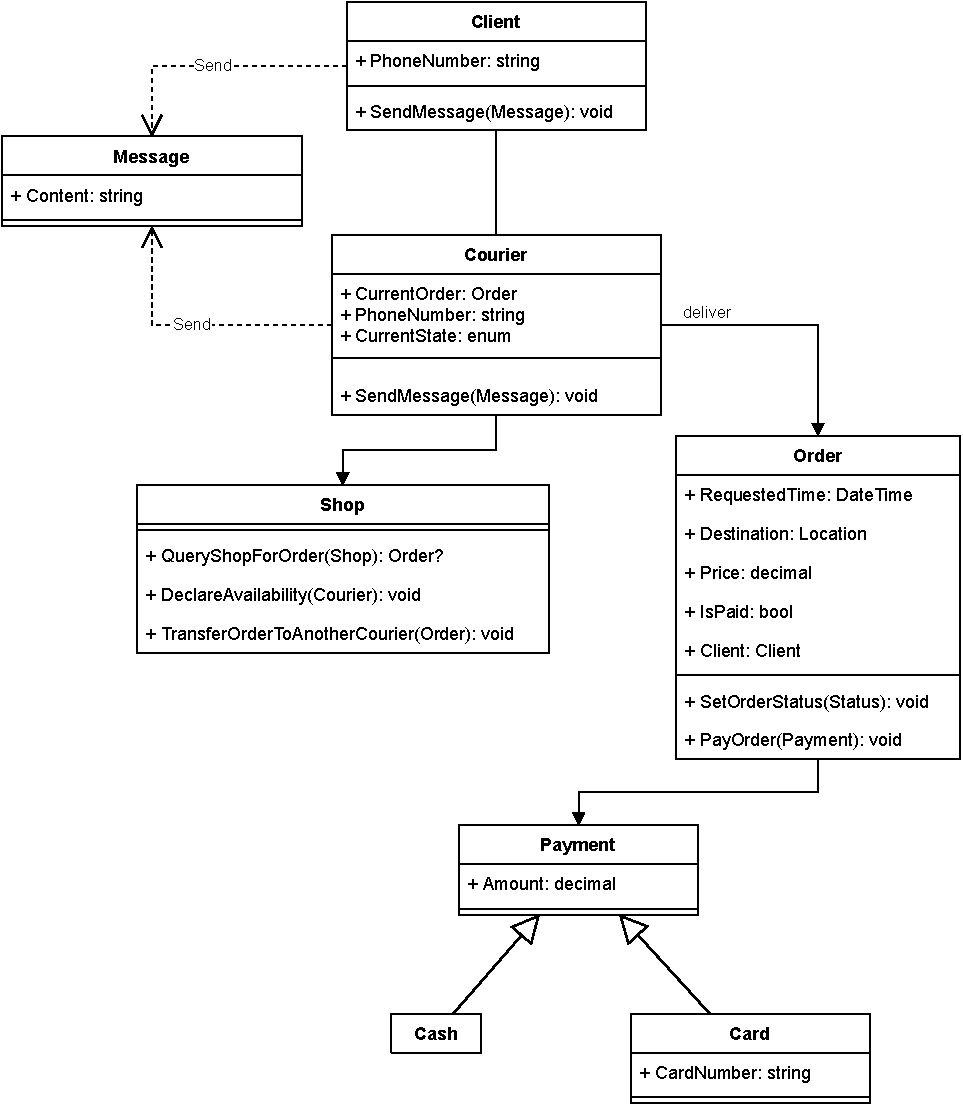
\includegraphics[width=1\textwidth]
{class-diagrams/delivery-class-diagram.pdf}
\end{figure}
\newpage


\subsubsection{Courier}

Courier is the main actor in delivery module. The courier is responsible for delivering the order from the shop to a client. That includes setting appropriate order status and collecting payment from clients, if they want to pay with cash. Besides that, courier can also communicate with the client by sending message or calling. If for some reason the courier can't deliver the products, the order can be transferred to another courier.

\subsubsection{Shop}

This class in delivery module represents the shop side in communicating with the courier, preceding the actual delivery. Through that class, courier can query the shop for new order or declare availability. If the courier is available, the shop can notify a courier, that the package is ready to be picked up. There is also a method providing information about a possibility of delegating the task to someone else when justified.

\subsubsection{Client}

In this module, the client is primarily used for communication between the courier and the client. There are two types of communication: over the phone and via text messages.

\subsubsection{Order}

Order object contains information, that is required for proper delivery of products. The order stores the delivery address (address of a client) and requested time (time, when the client wants to pick up the order from the courier). Additionally, order object has property \textbf{IsPaid}, which indicates, whether the Order has been paid (with card) or it will be paid with cash to the courier. Lastly, the order object has also reference to the Client object, which contains client details.

\end{document}